\chapter {Strongly coupled methods for coupled fields}

This chapter presents the most common strongly coupled/implicit methods employed to solve coupled field problems.
This presentation seeks to provide a literature overview of the available approaches.

% More thorough description of the chapter
Two main ways of realizing a strongly coupled approach to the solution of the coupled problem are presented.
The first focuses on fixed-point solvers and acceleration/stabilization techniques for them.
The second deals with approaches based on the Newton-Raphson method, with the main problem tackled being an efficient and accurate approximation to the Jacobian.\jvc{In the end, rewrite the description of the chapter}

\section{Equations to be solved}

For the sake of clarity, the discretized equations of the thermo-mechanical problem at the next time instant, \(n+1\)e are recovered here
\begin{gather}
    \mathbf M \ddot{\mathbf u}_{n+1} +\mathbf f_u^\text{\;int}(\bm \uptheta_{n+1}, \mathbf u_{n+1})-\mathbf f^\text{\;ext}_{u,n+1}=\mathbf 0, \label{eq:mech_problem} \\
    \mathbf C \dot{\bm \uptheta}_{n+1} +\mathbf f_\theta^\text{\;int}(\bm \uptheta_{n+1}, \mathbf u_{n+1})-\mathbf f^\text{\;ext}_{\theta,n+1}=\mathbf 0. \label{eq:therm_problem}
\end{gather}
The complete definition of the material incremental discretized thermo-mechanical initial boundary value problem can be found in Chapter~\ref{chapter:thermo_mechanical_problem}.

As only partitioned approaches are considered, the thermal and mechanical problems are solved separately, i.e., Equation~\eqref{eq:mech_problem} is solved considering a fixed temperature, and Equation~\eqref{eq:therm_problem} is solved assuming a fixed configuration.
To ease the discussion, consider the existence of two functions \(\pazocal U_{n+1}\) and \(\pazocal T_{n+1}\) that represent these solution procedures at timestep \(n+1\).
These so-called mechanical and thermal solvers satisfy
\begin{highlight}[innertopmargin=-5pt]
\begin{gather}
  \pazocal U\colon \mathscr K_{\theta, n+1}\to \mathscr K_{u,n+1},\quad \mathbf u = \pazocal U_{n+1}(\bm \uptheta),\\
  \pazocal T\colon \mathscr K_{u,n+1}\to \mathscr K_{\theta, n+1},\quad \bm \uptheta = \pazocal T_{n+1}(\mathbf u).
\end{gather}
\end{highlight}
See Chapter~\ref{chapter:thermo_mechanical_problem} for detailed information on them.
In the following, the subscripts on the solvers will be dropped to avoid clutter.

The goal now is to consider functions, built from \(\pazocal U\) and \(\pazocal T\), whose roots are also the solutions to the thermo-mechanical problem (Equations~\eqref{eq:mech_problem} and \eqref{eq:therm_problem}).
Several examples can be provided.
The most appropriate for the current use case are presented in what follows.
They can be found in \cite{uekermann_partitioned_2016} in the context of fluid-structure interaction (FSI).

Consider the residues defined as,
\begin{highlight}
\begin{equation} \label{eq:def_res_jacobi}
  \pazocal R_\text{J}\colon \mathscr K_{u,n+1}\times\mathscr K_{\theta,n+1} \to K_{u,n+1}\times\mathscr K_{\theta,n+1},\quad  \pazocal R_\text{J}(\mathbf u, \bm \uptheta) =
  \left\{\begin{array}{c}
  \mathbf u - \pazocal U(\bm \theta)\\
  \bm \uptheta - \pazocal T(\mathbf u)
  \end{array}\right\},
\end{equation}
\end{highlight}
and
\begin{highlight}
\begin{equation} \label{eq:def_res_gauss_seidel}
  \pazocal R_\text{GS}\colon \mathscr K_{\theta,n+1} \to\mathscr K_{\theta,n+1},\quad \pazocal R_\text{GS}(\bm \uptheta) =
  \bm \uptheta - \pazocal T\circ \pazocal U(\bm \uptheta),
\end{equation}
\end{highlight}
where the subscript "J" stands for Jacobi and the subscript "GS" for Gauss-Seidel.
The reason for this choice of subscripts is made clear in Section~\ref{sec:fixed_point_approach}.


Since the methods described below for the solution of nonlinear systems of equations apply to both functions \(\pazocal R_\mathrm{J}\) and \(\pazocal R_\mathrm{GS}\), a general function denoted as \(\pazocal R\), whose variable is \(\mathbf x\), is considered instead.
As already stated, the solution for the thermo-mechanical problem (Equations~\eqref{eq:mech_problem} and \eqref{eq:therm_problem}) can be abstracted as the solution of
\begin{equation} \label{eq:abstract_residue_equation}
  \pazocal R(\mathbf x) = 0.
\end{equation}
To obtain simpler expressions in what follows, consider also the function
\begin{equation}
\pazocal S(\mathbf x) = \mathbf x - \pazocal R(\mathbf x),
\end{equation}
whose fixed point is the solution to the nonlinear system of equation in Equation~\eqref{eq:abstract_residue_equation}.

\section{A classification scheme for iterative methods}

Most methods available for the solution of systems of nonlinear equations, such as the one in Equation~\eqref{eq:abstract_residue_equation}, are iterative methods.
They can be more precisely defined lettting \(\mathbf x^{k},\mathbf x^{k-1}, \ldots\), whose superscripts correspond to the loop of the iteration method, be approximants to \(\mathbf x_{n+1}\), whose subscript concerns the timestep

To better understand the landscape of available methods to solve nonlinear systems of equations, the iteration functions are classified according to the information they require following the classification scheme by \cite{traub_iterative_1982}.
Let \(\mathbf x^{k+1}\) be determined uniquely by information obtained at \(\mathbf x^{k}, \mathbf x^{k-1}, \ldots\), including the derivatives of any order of \(\pazocal R\).
Let the function that maps \(\mathbf x^{k}, \mathbf x^{k-1}, \ldots\) into \(\mathbf x^{k+1}\) be called \(\phi\).
Thus
\begin{highlight}
\begin{equation}
  \mathbf x^{k+1}=\phi\left(\mathbf x^{k},\pazocal R(\mathbf x^{k}), J_\pazocal{R}(\mathbf x^k), \dots\right),
\end{equation}
\end{highlight}
where \(\phi\) is called an iteration function, and \(J_\pazocal{R}\) is the Jacobian of \(\pazocal R\).
To prevent clutering \(\mathbf x^k\) will stand for its value as well as for the values of \(\pazocal R(\mathbf x^k)\), \(J_\pazocal{R}(\mathbf x^k)\) and further derivatives of higher order.
Then \(\phi\) is called a \textit{one-point iteration function}.
Most iteration functions that have been used for root-finding are one-point iteration functions. The most commonly known examples are the fixed point schemes and Newton's iteration method.

Next, let \(\mathbf x^{k+1}\) be determined by new information at \(\mathbf x^{k}\) and reused information at \(\mathbf x^{k-1}, \ldots\).
Thus
\begin{highlight}
  \begin{equation}\label{eq:one_point_iteration_function_with_memory}
    \mathbf x^{k+1}=\phi\left(\mathbf x^{k} ; \mathbf x^{k-1}, \ldots\right) .
  \end{equation}
\end{highlight}
Then \(\phi\) is called a \textit{one-point iteration function with memory}.
The semicolon in Equation~\eqref{eq:one_point_iteration_function_with_memory} separates the point at which new data are used from the points at which old data are reused.
The secant iteration function is the best-known example of a one-point iteration function with memory.

Let \(\mathbf x^{k+1}\) be determined by new information at \(\mathbf x^{k}, \omega_{1}\left(\mathbf x^{k}\right), \ldots\), \(\omega_{i}\left(\mathbf x^{k}\right)\), \(i \geq 1\), where \(\omega_i\) denote operations on \(\mathbf x^k\).
No old information is reused.
Thus
\begin{highlight}
  \begin{equation}
    \mathbf x^{k+1}=\phi\left[\mathbf x^{k}, \omega_{1}\left(\mathbf x^{k}\right), \ldots, \omega_{i}\left(\mathbf x^{k}\right)\right].
  \end{equation}
\end{highlight}
Then \(\phi\) is called a \textit{multipoint iterative function}.
Such methods include the Aitken-Steffson method.

Finally, let \(\mathbf z_{j}\) represent the quantities \(\mathbf x^{j}, \omega_{1}\left(\mathbf x^{j}\right), \ldots, \omega_{i}\left(\mathbf x^{j}\right)\), \(i \geq 1\).
Let
\begin{highlight}
  \begin{equation} \label{eq:multipoint_iterative_function_with_memory}
  \mathbf x^{k+1}=\phi\left(\mathbf z^{k} ; \mathbf z^{k-1}, \dots \right) .
  \end{equation}
\end{highlight}
Then \(\phi\) is called a \textit{multipoint iterative function with memory}.
The semicolon in Equation~\eqref{eq:multipoint_iterative_function_with_memory} separates the points at which new data are used from the points at which old data are reused.

In the present work, the criteria used for the choice of the iterative method used fit roughly into the ones provided by \cite{fang_two_2009} for problems in the context the electronic structure problems.
They are
\begin{enumerate}
  \item The dimensionality of the problem is large.
  \item \(\pazocal R(\mathbf x)\) is continuously differentiable, but the analytic form of its derivative is not readily available, or it is costly to compute.
  \item The cost of evaluating \(\pazocal R(\mathbf x)\) is computationally high.
  \item The problem is noisy. In other words, the evaluated function values of \(\pazocal R(\mathbf x)\) usually contain errors.
\end{enumerate}
Thus, the methods chosen must minimize the number of calls to \(\pazocal R\), as it is expensive to compute.
The amount of information saved from previous iterations must also be judiciously chosen as the problem's dimensionality is large, which can lead to memory limitation.
Finally, the analytical form of the derivative \(\pazocal{R}\) is also not available.
Thus methods that use it must be discarded.

\subsection{Predictor}

Iterative procedures are considered to solve the thermo-mechanical problem at a given timestep \(n+1\).
As the first value approximating \(\mathbf x_{n+1}\), one can employ the converged value of the previous timestep, \(\mathbf x_n\).
However, a very efficient way to increase the chances of stability and reduce computation time is to predict the optimal initial values at the beginning of every time step \citep{erbts_accelerated_2012, erbts_partitioned_2015, wendt_partitioned_2015}.
The prediction of the new solution by polynomial extrapolation is based on the converged solution of the last two or three timesteps.
This method is based on polynomial vector extrapolation, which is relatively easy to implement, and the extra computational input is negligible.

The maximum polynomial under consideration is of the order two, i.e., the new solution is extrapolated from the results from the last three time steps.
The predictors $\mathbf{x}^{*}$ for the order $p=1$ and $p=2$ polynomials read:
\begin{highlight}[innertopmargin=-5pt]
\begin{gather}
p=1:\quad \mathbf{x}_{n+1}^{*}=2 \mathbf{x}_{n}-\mathbf{x}_{n-1}, \\
p=2:\quad \mathbf{x}_{n+1}^{*}=3 \mathbf{x}_{n}-3 \mathbf{x}_{n-1}+\mathbf{x}_{n-2}.
\end{gather}
\end{highlight}

\subsection{Convergence criteria}

For an iterative method to be useful, there must be reasonable criteria to determine its convergence.
The iteration residual is defined as
\begin{equation}
\mathbf r^{k} = \pazocal R(\mathbf x^{k}),
\end{equation}
and if it is equal to zero then $\mathbf x$ is the solution to the system of nonlinear equations, i.e.,
\begin{equation} \label{eq:residual_definition}
\mathbf r = \pazocal R(\mathbf x) = \mathbf 0,
\end{equation}
and hence, a reasonable convergence measure for the iteration procedure.

The discrete  $l^{2}$-norm can be used to obtain a scalar representative of the vectorial residual \(\mathbf r^{k}=\left(r^{k,1}, \ldots, r^{k,m}\right)^{T}\) as
\begin{equation} \label{eq:absolute_residual_criterion}
\left\|\mathbf{r}^{k}\right\|_{L^{2}}=\sqrt{\sum_{i}\left(r^{k, i}\right)^{2}}.
\end{equation}

Directly using \eqref{eq:absolute_residual_criterion} yields an absolute convergence criterion
\begin{equation}
\left\|\boldsymbol{r} ^{k}\right\|_{l^{2}}<\epsilon_\mathrm{abs}.
\end{equation}
with $\epsilon_\mathrm{abs}>0$ as absolute convergence limit and convergence being obtained when the above condition renders valid.
However, since the absolute value of the $r^{k, i} $'s can change by orders of magnitude during one simulation, an absolute measure is not appropriate in all situations.
A relative measure solves this problem by setting the residual in relation with the current coupling iterate values as
\begin{equation}
\frac{\left\|\mathbf{r}^{k}\right\|_{l^{2}}}{\left\|\mathbf{x}^{k}\right\|_{l^{2}}}<\epsilon_\mathrm{rel}.
\end{equation}

A relative convergence measure can fail to work correctly when the coupling iterate values are close to zero, and rounding errors occur.
Thus, a combination of absolute and relative measures, where the absolute measure takes care of close to zero cases, and the relative handles all other cases, is often a good choice.



\section{One-point iteration function}

\subsection{Fixed-point approaches} \label{sec:fixed_point_approach}

The application of the fixed-point method to obtain the roots of \(\pazocal R\) yields
\begin{equation}
  \mathbf x^{k+1} = \pazocal S(\mathbf x^k) = \mathbf x^k - \pazocal R(\mathbf x^k).
\end{equation}
See Figure~\ref{fig:fixed_point_iteration} for its geometric interpretation in one dimension.

\begin{figure}
  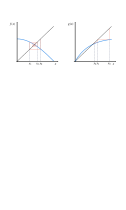
\includegraphics{figures/fixed_point_iteration}
  \caption{Geometric interpretation of the fixed-point iteration method in one dimension for two example functions \(f\) and \(g\).}
  \label{fig:fixed_point_iteration}
\end{figure}

If the particular functions defined on Equations~\eqref{eq:def_res_jacobi} and \eqref{eq:def_res_gauss_seidel} are used, one finds the  two basic Schwarz procedures commonly employed in strongly coupled solution procedures.
They are the additive or block Jacobi and the parallel Scharwz or Gauss-Seidel procedures.
The names originate from domain decomposition, and justify the subscripts employed in Equations~\eqref{eq:def_res_jacobi} and \eqref{eq:def_res_gauss_seidel}.

\subsubsection{Block Jacobi or Schwarz additive}

Applying the fixed-point approach to \(\pazocal R_\mathrm{J}\) (Equation~\eqref{eq:def_res_jacobi}), yields
\begin{align}
  \left\{\mathbf u^{k+1}, \bm\uptheta^{k+1}\right\}^T &= \pazocal S_\mathrm{J}(\mathbf u^k, \bm\uptheta^k)\\
   &= \left\{\mathbf u^k, \bm\uptheta^k\right\}^T - \pazocal R_\mathrm{J}(\mathbf u^k, \bm \uptheta^k),
\end{align}
It is the same as solving both the mechanical (Equation~\eqref{eq:mech_problem}) and the thermal problem (Equation~\eqref{eq:therm_problem}) in parallel.
Such a procedure is said to be Schwarz additive or block Jacobi, refering to the similarities with the procedure for the solution of linear systems of equations with the same name i.e.,
\begin{gather}
\mathbf u^{k+1} = \pazocal U(\bm \uptheta^k),\\
\bm \uptheta^{k+1} = \pazocal T(\mathbf u^k).
\end{gather}

Box~\ref{box:block_jacobi} shows the pseudo-code for the block Jacobi approach.

\begin{framedbox}[htb]
  \caption{Additive Schwarz procedure, also called block Jacobi, for one timestep.}
  \label{box:block_jacobi}
  \begin{center}
    \begin{minipage}{0.9\textwidth}
    \begin{enumerate}[(i)]
    \item \(\mathbf u^0 = \mathbf u_{n}\)
    \item \(\bm \uptheta^0 = \bm \uptheta_n\)
    \item Set fixed-point counter to zero: \(k=0\)
    \item Enter the fixed-point loop
    \begin{enumerate}[(1)]
      \item Solve the mechanical problem at fixed temeperature \(\bm \uptheta^k\): \(\mathbf u^{k+1} = \pazocal U(\bm \uptheta^k)\)
      \item Solve the thermal problem at a fixed configuration \(\mathbf u^k\): \(\bm \uptheta^{k+1} = \pazocal T(\mathbf u^k)\)
      \item If the desired accuracy has not been reached, update \(k=k+1\) and go to step (1).

    \end{enumerate}
    \end{enumerate}
    \end{minipage}
  \end{center}
\end{framedbox}

\subsubsection{Block Gauss-Seidel or Schwarz multiplicative}

Applying the fixed-point approach to \(\pazocal R_\mathrm{GS}\) (Equation~\eqref{eq:def_res_jacobi}), yields
\begin{equation}
  \bm\uptheta^{k+1} = \pazocal S_\mathrm{GS}(\bm\uptheta^k) =  \bm\uptheta^k - \pazocal R_\mathrm{GS}(\bm \uptheta^k).
\end{equation}
Thus, the fields are solved sequentially, where the output of the first solver is the input of the second solver.
This the solution procedure is said to be Scharwz multiplicative or block Gauss-Seidel.
\begin{gather}
\mathbf u^{k+1}  = \pazocal U(\bm \uptheta^k),\\
\bm \uptheta^{k+1} = \pazocal T(\mathbf u^{k+1}).
\end{gather}
One of the fields must be chosen as the first, and this may be crucial \citep{joosten_analysis_2009}.
Here, the focus is on the sequence coinciding with the isothermic split, i.e., first, the mechanical problem is solved at a fixed temperature.
Then the thermal problem is solved at a fixed configuration.

Box~\ref{box:block_gauss_seidel} shows the pseudo-code for the block Gauss-Seidel approach.

\begin{framedbox}[htb]
  \caption{Multiplicative Schwarz procedure, also called block Gauss-Seidel, for one timestep.}
  \label{box:block_gauss_seidel}
  \begin{center}
    \begin{minipage}{0.9\textwidth}
    \begin{enumerate}[(i)]
    \item \(\mathbf u^0 = \mathbf u_{n}\)
    \item \(\bm \uptheta^0 = \bm \uptheta_n\)
      \item Set fixed-point counter to zero: \(k=0\)
    \item Enter the fixed-point loop
    \begin{enumerate}[(1)]
      \item Solve the mechanical problem at fixed temeperature \(\bm \uptheta^k\): \(\mathbf u^{k+1} = \pazocal U(\bm \uptheta^k)\)
      \item Solve the thermal problem at a fixed configuration \(\mathbf u^{k+1}\): \(\bm \uptheta^{k+1} = \pazocal T(\mathbf u^{k+1})\)
      \item If the desired accuracy has not been reached, update \(k=k+1\) and go to step (1).

    \end{enumerate}
    \end{enumerate}
    \end{minipage}
  \end{center}
\end{framedbox}

\subsection{Newton's method}

The Newton-Raphson or Newton scheme is a very popular iterative solution procedure for nonlinear systems of equations, which under appropriate conditions, converges quadratically.
It can be applied to Equation~\eqref{eq:abstract_residue_equation} yielding
\begin{highlight}[innertopmargin=-5pt]
  \begin{gather}
    J_\pazocal{R}(\mathbf x^k)\Delta \mathbf x^k = - \pazocal R(\mathbf x^k), \label{eq:newton_system}\\
    \mathbf x^{k+1} = \mathbf x^k + \Delta \mathbf x^k. \label{eq:newton_iter}
  \end{gather}
\end{highlight}
See Figure~\ref{fig:newton_method} for its geometric interpretation in one dimension.

\begin{figure}[htbp]
  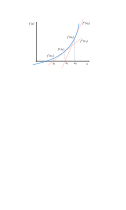
\includegraphics{figures/newton_method}
  \caption{Geometric interpretation of the Newton method in one dimension for an example function \(f\), whose derivative is denoted by \(f'\).}
  \label{fig:newton_method}
\end{figure}

In particular, using \(\pazocal R_\mathrm{J}\), a few simplifications can be obtained.
To ease the explanation, consider, a thermal residual operator $\pazocal{R}_{u}(\mathbf{u}, \bm{\uptheta})$ and a mechanical residual operator $\pazocal{R}_{\theta}(\mathbf{u}, \bm{\uptheta})$ defined to be the first and second components in the definition of \(\pazocal R_\mathrm{J}\) (Equation~\eqref{eq:def_res_gauss_seidel}).
Written in full
\begin{gather}
\pazocal{R}_{u}(\mathbf{u}, \bm{\uptheta})=\mathbf{u}-\pazocal{U}(\bm{\uptheta})=0, \\
\pazocal{R}_{\theta}(\mathbf{u}, \bm{\uptheta})=\bm{\uptheta}-\pazocal{T}(\mathbf{u})=0,
\end{gather}

From this, a block Newton iteration can be written as
\begin{highlight}
  \begin{equation} \label{eq:block_newton_raphson}
  \left[\begin{array}{l}
  J_{\pazocal{R}_{u}}\left(\mathbf u^k, \bm{\uptheta}^{k}\right) \\[7pt] J_{\pazocal{R}_{\theta}}\left(\mathbf{u}^{k}, \bm\uptheta^k\right)
  \end{array}\right]
  \left\{\begin{array}{c}\Delta \mathbf{u}^{k} \\ \Delta \bm{\uptheta}^{k}\end{array}\right\}
  =-\left\{\begin{array}{l}\pazocal{R}_{u}\left(\mathbf{u}^{k}, \boldsymbol{\theta}^{k}\right) \\ \pazocal{R}_{\theta}\left(\mathbf{u}^{k}, \boldsymbol{\theta}^{k}\right)\end{array}\right\},
  \end{equation}
\end{highlight}
and the update of the iteration variables reads
\begin{highlight}
  \begin{equation}
  \left\{\begin{array}{l}
  \mathbf{u}^{k+1} \\
  \boldsymbol{\theta}^{k+1}
  \end{array}\right\}=\left\{\begin{array}{l}
  \mathbf{u}^{k} \\
  \boldsymbol{\theta}^{k}
  \end{array}\right\}+\left\{\begin{array}{c}
  \Delta \mathbf{u}^{k} \\
  \Delta \boldsymbol{\theta}^{k}
  \end{array}\right\}.
  \end{equation}
\end{highlight}


The system of equations in Equation~\eqref{eq:block_newton_raphson} can be further simplified following \cite{degroote_development_2010} considering the definitions of the mechanical and thermal residuals and taking their derivatives.
It yields
\begin{equation}
\left[\begin{array}{cc}
\mathbf I & -J_{\pazocal{U}}\left(\bm{\uptheta}^{k}\right) \\[7pt]
-J_{\pazocal{T}}\left(\mathbf{u}^{k}\right) & \mathbf I
\end{array}\right]
\left\{\begin{array}{c}\Delta \mathbf{u}^{k} \\ \Delta \bm{\uptheta}^{k}\end{array}\right\}
=-\left\{\begin{array}{l}\pazocal{R}_{u}\left(\mathbf{u}^{k}, \boldsymbol{\theta}^{k}\right) \\ \pazocal{R}_{\theta}\left(\mathbf{u}^{k}, \boldsymbol{\theta}^{k}\right)\end{array}\right\},
\end{equation}

Solving for \(\Delta \mathbf u^k\) and \(\Delta \bm \uptheta^k\), one finds
\begin{align}
  \left(\mathbf I + J_\pazocal{U}(\bm\uptheta^k)J_\pazocal{T}(\mathbf u^k)\right)\Delta \mathbf u^k &= - \pazocal R_u(\mathbf u^k, \bm \uptheta^k)+J_\pazocal{U}(\bm\uptheta^k)\pazocal R_\theta(\mathbf u^k, \bm\uptheta^k), \label{eq:explicit_eq_delta_u_newton}\\
  \left(\mathbf I + J_\pazocal{T}(\mathbf u^k)J_\pazocal{U}(\bm\uptheta^k)\right)\Delta \bm\uptheta^k &= - \pazocal R_\theta(\bm \uptheta^k, \mathbf u^k)+J_\pazocal{\theta}(\mathbf u^k)\pazocal R_u(\mathbf u^k, \bm\uptheta^k). \label{eq:explicit_eq_delta_theta_newton}
\end{align}
Thus, the Jacobians now needed are \(J_\pazocal{U}\) and \(J_\pazocal{T}\).
See Section~\ref{sec:quasi_newton} for the practical application of this.

Every iteration of the Newton scheme involves at least one invocation of the thermal and mechanical solvers when computing $\pazocal{R}\left(\mathbf{u}^{k}\right)$ or both $\pazocal{R}_{u}\left(\mathbf{u}^{k}, \boldsymbol{\theta}^{k}\right)$ and $\pazocal{R}_{\theta}\left(\mathbf{u}^{k}, \boldsymbol{\theta}^{k}\right)$.
The critical point for black-box equation coupling is how to obtain the derivative information in the Jacobi matrices.
In different ways, some of the methods presented next find approximations for the required Jacobian times vector products.



\subsubsection{Constant Underrelaxation}

One of the most straightforward ways to stabilize an iterative method is to use constant underrelaxation \citep{gatzhammer_efficient_2014}.
The relaxation is performed as follows
\begin{equation} \label{eq:constant_relaxation}
\mathbf x^{k+1}=(1-\omega) \mathbf x^{k}+\omega\left(\mathbf x^k - \pazocal R(\mathbf x^k)\right)=\mathbf x^{k} -\omega \mathbf{r}^{k+1},
\end{equation}
where \(\omega\) is the relaxation factor chosen in the range \(0<\omega<1\), which corresponds to an underrelaxation, to achieve a stabilizing effect.

Applying to Equation~\eqref{eq:def_res_jacobi}
\begin{equation}
  \left\{\begin{array}{c}
    \mathbf u^{k+1}\\
    \bm \uptheta^{k+1}
  \end{array}\right\} =
  (1-\omega)
  \left\{\begin{array}{c}
    \mathbf u^{k}\\
    \bm \uptheta^{k}
  \end{array}\right\}
  + \omega
  \left\{\begin{array}{c}
    \pazocal U(\bm\uptheta^k)\\
    \pazocal T(\mathbf u^k)
  \end{array}\right\}
\end{equation}
Applying to Equation~\eqref{eq:def_res_gauss_seidel}
\begin{equation}
  \bm\uptheta^{k+1} = (1-\omega)\bm\uptheta^k + \omega \pazocal T\circ\pazocal U(\bm \uptheta^k).
\end{equation}


Constant underrelaxation works well if \(\omega\) is close to 1 but leads to a slow convergence if \(\omega\) has to be chosen close to 0.
Thus, the constant underrelaxation method creates unmanageable computational costs for severe instabilities.
The optimal \(\omega\) is not necessary the largest stable one \citep{gatzhammer_efficient_2014} and has to be set empirically.
In what follows, alternative methods are discussed, which try to decrease the number of iterations necessary while maintaining stability.

\begin{framedbox}[htb]
  \caption{Constant underrelaxation applied to the block Gauss-Seidel scheme.}
  \label{box:constant_underrelaxation}
  \begin{center}
    \begin{minipage}{0.9\textwidth}
    \begin{enumerate}[(i)]
    \item \(\bm\uptheta^0 = \bm\uptheta_{n+1}^p\)
    \item Set fixed-point counter to zero: \(k=0\)
    \item Enter the fixed-point loop
    \begin{enumerate}[(1)]
      \item Solve the mechanical problem at fixed temeperature \(\bm \uptheta^k\): \(\mathbf u^{k+1} = \pazocal U(\bm \uptheta^k)\)
      \item Solve the thermal problem at a fixed configuration \(\mathbf u^{k+1}\): \(\bm \uptheta^{k+1} = \pazocal T(\mathbf u^{k+1})\)
      \item Compute \(\bm \uptheta^{k+1}\) using constant relaxation (Equation~\eqref{eq:constant_relaxation})
      \item If the desired accuracy has not been reached, update \(k=k+1\) and go to step (1).
    \end{enumerate}
    \end{enumerate}
    \end{minipage}
  \end{center}
\end{framedbox}

\section{One-point iteration function with memory}

\subsubsection{Aitken relaxation}


The so-called Aitken \(\Delta^2\) relaxation method was introduced by \cite{irons_version_1969} as a modified Aitken \(\Delta^2\) that does not require the computation of the function twice per iteration as in the original method.
It has been widely used in the context of FSI \citep{irons_version_1969, kuttler_fixed-point_2008, joosten_analysis_2009, kuttler_vector_2009, erbts_partitioned_2015, wendt_partitioned_2015}.
It has also been used in the context of thermo-mechanics by \cite{danowski_monolithic_2013}.

In the one-dimensional case, this method resembles the secant method applied to the fixed point problem, which can be used to solve nonlinear equations without differentiation.
Calling it an Aitken method is perhaps a misnomer since, in the Aitken-Steffensen method, the function values are computed twice per iteration.
It is more closely related to secant methods, reusing values from previous iterations.
This version of Aitken's \(\Delta^2\) method provides a dynamic under relaxation, which can be used to improve the convergence/stability properties of the coupling algorithm.

Assume that \(f\) is the function whose fixed point is sought.
The linear interpolation between two points already known of the function, \((a, f(a))\) and \((b, f(b)\) is
\begin{equation}
  y = \frac{f(b)-f(a)}{b-a}(x-a) + f(a).
\end{equation}
The fixed point of this approximation is
\begin{equation}
  c = \frac{f(b)-f(a)}{b-a}(c-a) + f(a).
\end{equation}
Thus, after rearranging,
\begin{equation}\
c=\frac{a f(b)- b f(a)}{\left(a-f(a)\right)-\left(b-f(b)\right)}
\end{equation}
This can be rewritten as
\begin{equation}
c=\left(1-\omega_{b}\right) b+\omega_{b} f(b) \quad \text { with } \omega_{b}=\frac{a-b}{\left(a-f(a)\right)-\left(b-f(b)\right)}
\end{equation}

The difference \(f(b)-f(a)\) is computationally inconvenient.\jvc{Why?}
Anticipating the next iteration step,
\begin{equation}
d=\left(1-\omega_{c}\right) c+\omega_{c} f(c) \quad \text { with } \omega_{c}=\frac{c-b}{\left(b-f(b)\right)-\left(c-f(c)\right)}
\end{equation}
a convenient expression for updating the relaxation factor may be found, i.e.
\begin{equation}
\omega_{c}=-\omega_{b}\frac{f(b)-b}{(c-f(c))-(f(b)-b)}.
\end{equation}
See Figure~\ref{fig:mod_aitken} for its geometric interpretation in one dimension.

\begin{figure}[htbp]
  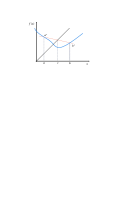
\includegraphics{figures/mod_aitken}
  \caption{Geometric interpretation of the Aitken relaxation in one dimension for an example function \(f\).}
  \label{fig:mod_aitken}
\end{figure}

Now, for the vector case, the next step is to work out the solution to the current iteration from the outcome of the previous iteration $\mathbf{x}^{(k)}$ plus a new increment $\Delta \mathbf{x}^{(k)}$
\begin{equation}
\mathbf{x}^{(k+1)}=\mathbf{x}^{(k)}+\Delta \mathbf{x}^{(k)}.
\end{equation}
The increment reads
\begin{equation}
\Delta \mathbf{x}^{(k)}=\omega^{(k)}\left(\pazocal S(\mathbf{x}^{(k)})-\mathbf{x}^{(k)}\right)=-\omega^{(k)} \mathbf r^{(k)}.
\end{equation}
with $\omega^{(k)}$ being the relaxation coefficient.
This coefficient is updated in every iteration cycle as a function of two previous residuals
\begin{highlight}
  \begin{equation}
    \omega^{(k)}=-\omega^{(k-1)} \frac{\left(\mathbf{r}^{(k)}-\mathbf{r}^{(k-1)}\right)^{\mathrm{T}} \mathbf{r}^{(k-1)}}{\left(\mathbf{r}^{(k)}-\mathbf{r}^{(k-1)}\right)^{2}}.
  \end{equation}
\end{highlight}\jvc{Check signs!!!}
Comparing with Equations~\eqref{eq:newton_system} and \eqref{eq:newton_iter}, \(\omega^{(k)}\) can be, in a sense, regarded as an approximation to the inverse of the Jacobian.
Dynamic relaxation is also easy to implement, and the additional computational input is acceptable since only inner vector products must be performed.

\subsection{Broyden's method and Broyden's family}

The following exposition follows closely \cite{fang_two_2009}.
In quasi-Newton methods the Jacobian is updated in each iteration using a rank-one update.
Standard quasi-Newton methods require the updated \(J_{k+1}\) to satisfy the following secant condition
\begin{equation} \label{eq:secant_condition}
J_\pazocal{R}^{k+1} \Delta \mathbf x^{k}=\Delta \pazocal R^{k},
\end{equation}
where \(\Delta \pazocal R^{k}\equiv \pazocal R\left(\mathbf x^{k+1}\right)-\pazocal R\left(\mathbf x^ {k}\right)\).
Furthermore, another common requirement is the following so-called no-change condition
\begin{equation} \label{eq:no_change_condition}
J_\pazocal R^{k+1} \mathbf q=J_\pazocal R^{k} \mathbf q \quad \forall \mathbf q \text { such that } \mathbf q^{\mathrm{T}} \Delta \mathbf x^{k}=0,
\end{equation}
which stipulates that there be no new information from \(J_\pazocal R^{k}\) to \(J_\pazocal R^{k+1}\) along any direction \(\mathbf q\) orthogonal to \(\Delta \mathbf x^{k}\).

\cite{broyden} developed a method satisfying both secant condition (Equation~\eqref{eq:secant_condition}) and the no-change condition (Equation~\eqref{eq:no_change_condition}).
By simply imposing these conditions he arrived at the update formula
\begin{highlight}
\begin{equation} \label{eq:good_update_broyden}
J_{\pazocal R}^{k+1}=J_{\pazocal R}^{k}+\left(\Delta \pazocal R^{k}-J_{\pazocal R}^{k} \Delta \mathbf x^{k}\right) \frac{\Delta {\mathbf x^{k}}^{\mathrm{T}}}{\Delta {\mathbf x^{k}}^{\mathrm{T}} \Delta \mathbf x^{k}}.
\end{equation}
\end{highlight}

Matrix \(J_\pazocal R^{k+1}\) in Equation~\eqref{eq:good_update_broyden} is the unique matrix satisfying both conditions \eqref{eq:secant_condition} and \eqref{eq:no_change_condition}.
The Broyden update can also be obtained by minimizing \(E\left(J_\pazocal R^{k+1}\right)=\left\|J_\pazocal R^{k+1}-J_\pazocal R^{k}\right\|_{F}^{2}\) with respect to terms of \(J_\pazocal R^{k+1}\), subject to the secant condition \eqref{eq:secant_condition}.

It may seem at first that Broyden's first method can be expensive since computing the quasi-Newton step \(\Delta \mathbf x^{k}\) requires solving a linear system at each iteration.
However, note that, typically, the approximate Jacobian is a small rank modification of a diagonal matrix (or a matrix that is easy to invert); hence, the cost to obtain this solution is not too high as long as the number of steps is not too large.

An alternative is Broyden's second method that approximates the inverse Jacobian instead of the Jacobian itself.
\(G_\pazocal R^{k}\) is used to denote the estimated inverse Jacobian at the \(k\) th iteration.
The secant condition (Equation~\eqref{eq:secant_condition}) now reads
\begin{equation} \label{eq:inverse_secant_cond}
G_\pazocal R^{k+1} \Delta \pazocal R^{k}=\Delta \mathbf x^{k}
\end{equation}
By minimizing \(E\left(G_\pazocal R^{k+1}\right)=\left\|G_\pazocal R^{k+1}-G_\pazocal R^{k}\right\|_{F}^{2}\) with respect to \(G_\pazocal R^{k+1}\) subject to Equation~\eqref{eq:inverse_secant_cond}, the following update formula is found for the inverse Jacobian
\begin{highlight}
  \begin{equation} \label{eq:bad_update_broyden}
  G_\pazocal R^{k+1}=G_\pazocal R^{k}+\left(\Delta \mathbf x_{k}-G_\pazocal R^{k} \Delta \pazocal R^{k}\right) \frac{\Delta {\pazocal R^{k}}^{\mathrm{T}}}{\Delta {\pazocal R^{k}}^{\mathrm{T}} \Delta \pazocal R^{k}}
  \end{equation}
\end{highlight}
which is also the only update satisfying both the secant condition (Equation~\eqref{eq:inverse_secant_cond}) and the no-change condition for the inverse Jacobian
\begin{equation}
  G_\pazocal R^{k} \mathbf q=G_\pazocal R^{k+1} \mathbf q \quad \forall \mathbf q \text { such that } \mathbf q^{\mathrm{T}} \Delta \pazocal R^{k}=0.
\end{equation}
The update formula in Equation~\eqref{eq:good_update_broyden} can also be obtained in terms of \(G_\pazocal R^{k} \equiv {J_\pazocal R^{k}}^{-1}\) by applying the Sherman-Morrison formula
\begin{equation}
G_\pazocal R^{k+1}=G_\pazocal R^{k}+\left(\Delta \mathbf x^{k}-G_\pazocal R^{k} \Delta \pazocal R^{k}\right) \frac{\Delta {\mathbf x^{k}}^{\mathrm{T}} G_\pazocal R^{k}}{\Delta {\mathbf x^{k}}^{\mathrm{T}} G_\pazocal R^{k} \Delta \pazocal R^{k}}
\end{equation}
This shows, as was explained earlier, that to solve the Jacobian system associated with Broyden's first approach can be reduced to a set of update operations that are not more costly than those required by the second update.
Note, however, that the above formula requires the inverse of the initial Jacobian.

From Equation~\eqref{eq:good_update_broyden} and Equation~\eqref{eq:bad_update_broyden} it is possible to define Broyden's family of updates, in which an update formula takes the general form
\begin{equation}
G_\pazocal R^{k+1}=G_\pazocal R^{k}+\left(\Delta \mathbf x^{k}-G_\pazocal R^{k} \Delta \pazocal R^{k}\right) \mathbf v_{k}^{\mathrm{T}}
\end{equation}
where \(\mathbf v_{k}^{\mathrm{T}} \Delta \pazocal R^{k}=1\) so that the secant condition \eqref{eq:secant_condition} holds.
Note that the secant condition \eqref{eq:inverse_secant_cond} is equivalent to condition \eqref{eq:secant_condition}.
The pseudo-code of Broyden's two methods is given in Box~\ref{}.
Some authors called Broyden's first method Broyden's good update and Broyden's second method as Broyden's bad update.
These are two particular members of Broyden's family.

% \subsubsection{Steepest Descent Relaxation}
%
% In [97], a steepest descent-based relaxation method is investigated. The goal is to find an optimal value \(\omega_{k}\) for every iteration \(k\) and to use it in the relaxation (2.112). A convex scalar merit function \(\phi(\boldsymbol{s})\) is assumed to exist, to be minimal at the solution \(\boldsymbol{s}^{n+1}\), and to be sufficiently smooth. This merit function is not defined in [97]. Only its derivative is used within the algorithm, defined as the coupling iteration residual.
% \[
% \phi^{\prime}\left(\boldsymbol{s}_{k}\right):=\boldsymbol{r}_{k+1},
% \]
%
% such that \(\phi^{\prime}\left(s^{n+1}\right)=\mathbf{0}\). Using the merit function, an optimal relaxation factor can be found by
% \[
% \omega_{k}=\underset{\omega}{\arg \min } \phi\left(\boldsymbol{s}_{k}+\omega \boldsymbol{r}_{k+1}\right)
% \]
% and a sufficient condition for the optimal \(\omega_{k}\) is given by
% \[
% \frac{d \phi}{d \omega_{k}}=\left(\phi^{\prime}\left(\boldsymbol{s}_{k}+\omega_{k} \boldsymbol{r}_{k+1}\right)\right)^{T} \boldsymbol{r}_{k+1} \stackrel{!}{=} \mathbf{0} .
% \]
% An approximation for the optimal relaxation factor can be obtained from a truncated Taylor expansion of its first derivative
% \[
% \phi^{\prime}\left(\boldsymbol{s}_{k}+\omega_{k} \boldsymbol{r}_{k+1}\right) \approx \underbrace{\phi^{\prime}\left(\boldsymbol{s}_{k}\right)}_{=\boldsymbol{r}_{k+1}}+\omega_{k} \phi^{\prime \prime}\left(\boldsymbol{s}_{k}\right) \boldsymbol{r}_{k+1},
% \]
% where \(\phi^{\prime \prime}\left(s_{k}\right)\) is the symmetric matrix of second order partial derivatives of \(\phi\left(s_{k}\right)\) or the Jacobian of \(r_{k}\) with respect to \(s_{k}{ }^{5}\) Transposing (2.133) and multiplying it from the right with \(r_{k+1}\), the optimal relaxation factor can be obtained by
% \[
% \omega_{k}=-\frac{\left(\boldsymbol{r}_{k+1}\right)^{T} \boldsymbol{r}^{k+1}}{\left(\boldsymbol{r}^{k+1}\right)^{T} J_{\boldsymbol{r}_{k}}(\boldsymbol{s}) \boldsymbol{r}_{k+1}} .
% \]
% The remaining problem is how to determine the interface Jacobian \(J_{r_{k}}(s)\) since it is not accessible when black-box solvers are used. Two approximations for the matrix-vector product \(J_{\boldsymbol{r}_{k}}(s) \boldsymbol{r}_{k+1}\) are proposed in [97]. The first approximation is obtained by using a finite difference approach as
% \[
% J_{\boldsymbol{r}_{k}}(\boldsymbol{s}) \boldsymbol{y} \approx \frac{\boldsymbol{S} \circ \boldsymbol{F}\left(\boldsymbol{s}_{k}+\delta \boldsymbol{y}\right)-\boldsymbol{s}_{k}-\delta \boldsymbol{y}-\boldsymbol{r}_{k+1}}{\delta},
% \]
% with
% \[
% \delta=\frac{\lambda\left(\lambda+\left\|\boldsymbol{s}_{k}\right\|_{L_{2}}\right)}{\left\|\boldsymbol{r}_{k+1}\right\|_{L_{2}}}
% \]
% and \(\lambda\) chosen small enough \({ }^{6}\). The evaluation (2.135) needs one more call of fluid and structure solvers per coupling iteration. To decrease the computational costs for the extra evaluation, it is proposed to reduce the accuracy of the field solvers.
% The second approximation uses approximated fluid derivatives and exact structure derivatives, which are not available for black-box coupling and, thus, this alternative is not considered here.

\subsection{Multi-secant methods}

The multi-secant methods provide an approximation to the Jacobian in Equation~\eqref{eq:newton_system} or Equation~\eqref{eq:block_newton_raphson} using information from previous iterations.


\subsubsection{Generalized Broyden}

A generalized Broyden's method with a flexible rank update on the inverse Jacobian, satisfying a set of \(m\) secant equations
\begin{equation} \label{eq:multi_secant_eqs}
  G_\pazocal R^{k} \Delta \pazocal R^{i}=\Delta \mathbf x^{i} \quad \text { for } i=k-m, \ldots, k-1
\end{equation}
where it is assumed \(\Delta \pazocal R^{k-m}, \ldots, \Delta \pazocal R^{k-1}\) are linearly independent and \(m \leqslant n\) can also be described.
Aggregating Equations~\eqref{eq:multi_secant_eqs} in matrix form, they can be rewriten it as
\begin{equation} \label{eq:multi_secant_eqs_mat}
  G_\pazocal R^{k} \mathscr{R}^{k}=\mathscr{X}^{k}.
\end{equation}
where
\begin{equation}
\mathscr{R}^{k}=\left[\Delta \pazocal R^{k-m} \cdots \Delta \pazocal R^{k-1}\right], \quad \mathscr{X}^{k}=\left[\Delta \mathbf x^{k-m} \cdots \Delta \mathbf x^{k-1}\right] \in \mathbb{R}^{n \times m}
\end{equation}
The no-change condition corresponding to \eqref{eq:no_change_condition} is
\begin{equation}
  \left(G_\pazocal R^{k}-G_\pazocal R^{k-m}\right) \mathbf q=0
\end{equation}
for all \(\mathbf q\) orthogonal to the subspace spanned by \(\Delta \pazocal R^{k-m}, \ldots, \Delta \pazocal R^{k-1}\), the columns of \(\mathscr{R}^{k}\).
In the end, this yields
\begin{equation}
  G_\pazocal R^{k}=G_\pazocal R^{k-m}+\left(\mathscr{X}^{k}-G_\pazocal R^{k-m} \mathscr{R}^{k}\right)\left({\mathscr{R}^{k}}^{\mathrm{T}} \mathscr{R}^{k}\right)^{-1} {\mathscr{R}^{k}}^{\mathrm{T}}
\end{equation}
a rank-\(m\) update formula.
Note that \(\operatorname{rank}\left(\mathscr{R}^{k}\right)=m\).
The update formula for \(\mathbf x^{k+1}\) is
\begin{align}
\mathbf x^{k+1} &=\mathbf x^{k}-G_\pazocal R^{k} \pazocal R^{k} \\
&=\mathbf x^{k}-G_\pazocal R^{k-m} \pazocal R^{k}-\left(\mathscr{X}^{k}-G_\pazocal R^{k-m} \mathscr{R}^{k}\right)\left({\mathscr{R}^{k}}^{\mathrm{T}} \mathscr{R}^{k}\right)^{-1} {\mathscr{R}^{k}}^{\mathrm{T}} \pazocal R^{k} \\
&=\mathbf x^{k}-G_\pazocal R^{k-m} \pazocal R^{k}-\left(\mathscr{X}^{k}-G_\pazocal R^{k-m} \mathscr{R}^{k}\right) \gamma_{k} \label{eq:update_gen_broyden_ls}
\end{align}
where the column vector \(\gamma_{k}\) is obtained by solving the normal equations \(\left({\mathscr{R}^{k}}^{\mathrm{T}} \mathscr{R}^{k}\right) \gamma_{k}={\mathscr{R}^{k}}^{\mathrm{T}} \pazocal R^{k}\), which is equivalent to solving the least squares problem
\begin{equation}
  \min _{\gamma}\left\|\mathscr{R}^{k} \gamma-\pazocal R^{k}\right\|_{2}
\end{equation}
Note that in Equation~\eqref{eq:update_gen_broyden_ls}, if \(\mathscr{R}^{k}\) is square and of full rank, then for any \(G_\pazocal R^{k-m}\),
\begin{equation}
  \mathbf x^{k+1}=\mathbf x^{k}-\mathscr{X}^{k} {\mathscr{R}^{k}}^{-1} \pazocal R^{k}
\end{equation}
the same form as that in the standard secant method.

\subsubsection{Anderson mixing}

The Anderson mixing scheme [5] takes the latest \(m\) steps into account to obtain a better approximation to \(\mathbf x_{n+1}\) without evaluating \(\pazocal R\) again.
Consider
\begin{align}
  \bar{\mathbf x}^{k}=\mathbf x^{k}-\sum_{i=k-m}^{k-1} \gamma_{i}^{k} \Delta \mathbf x^{i}=\mathbf x_{k}-\mathscr{X}^{k} \gamma^{k}, \label{eq:anderson_x_bar}\\
  \bar{\pazocal R}^{k}=\pazocal R^{k}-\sum_{i=k-m}^{k-1} \gamma_{i}^{k} \Delta \pazocal R^{i}=\pazocal R^{k}-\mathscr{R}^{k} \gamma^{k} \label{eq:anderson_r_bar},
\end{align}
where \(\Delta \mathbf x^{i}=\mathbf x^{i+1}-\mathbf x^{i}\) and \(\Delta \pazocal R^{i}=\pazocal R^{i+1}-\pazocal R^{i}\), \(\mathscr{X}^{k}=\left[\Delta \mathbf x^{k-m} \cdots \Delta \mathbf x^{k-1}\right]\), \(\mathscr{R}^{k}=\left[\Delta \pazocal R^{k-m} \cdots \Delta \pazocal R^{k-1}\right]\), and \(\gamma^{k}=\left[\gamma_{k-m}^{k} \cdots \gamma_{k-1}^{k}\right]^{\mathrm{T}}\).
Expressing the equations in the form \(\bar{\mathbf x}^{k}=\sum_{j=k-m}^{k} w_{j} \mathbf x^{j}\) and \(\bar{\pazocal R}^{k}=\sum_{j=k-m}^{k} w_{j} \pazocal R^{j}\), it is found that \(\sum_{j=k-m}^{k} w_{j}=1\).
In other words, \(\bar{\mathbf x}_{k}\) and \(\bar{\pazocal R}_{k}\) are weighted averages of \(\mathbf x_{k-m}, \ldots, \mathbf x_{k}\) and \(\pazocal R^{k-m}, \ldots, \pazocal R^{k}\), respectively.
The arguments \(\gamma^{k}=\left[\gamma_{k-m}^{k} \cdots \gamma_{k-1}^{(k)}\right]^{\mathrm{T}}\) are determined by minimizing
\begin{equation}
E\left(\gamma^{k}\right)=\left\langle\bar{\pazocal R}^{k}, \bar{\pazocal R}^{k}\right\rangle=\left\|\pazocal R^{k}-\mathscr{R}^{k} \gamma^{k}\right\|_{2}^{2}
\end{equation}
whose solution can, but should not in practice, be obtained by solving the normal equations
\begin{equation}
\left({\mathscr{R}^{k}}^{\mathrm{T}} \mathscr{R}^{k}\right) \gamma^{k}={\mathscr{R}^{k}}^{\mathrm{T}} \pazocal R^{k}. \label{eq:normal_eqs_anderson}
\end{equation}
Combining Equations~\eqref{eq:anderson_x_bar}, \eqref{eq:anderson_r_bar}, and \eqref{eq:normal_eqs_anderson}, one obtains
\begin{align}
\mathbf x^{k+1} &=\bar{\mathbf x}^{k}+\beta \bar{\pazocal R}^{k} \\
&=\mathbf x^{k}+\beta \pazocal R^{k}-\left(\mathscr{X}^{k}+\beta \mathscr{R}^{k}\right) \gamma^{k} \\
&=\mathbf x^{k}+\beta \pazocal R^{k}-\left(\mathscr{X}^{k}+\beta \mathscr{R}^{k}\right)\left({\mathscr{R}^{k}}^{\mathrm{T}} \mathscr{R}^{k}\right)^{-1} {\mathscr{R}^{k}}^{\mathrm{T}} \pazocal R^{k} \label{eq:update_anderson_mixing}
\end{align}
where \(\beta\) is the preset mixing parameter and \({\mathscr{R}^{k}}^{\mathrm{T}} \mathscr{R}^{k}\) is assumed to be nonsingular.
In particular, if no previous iterate is taken into account (i.e. \(m=0\) ), then Equation~\eqref{eq:update_anderson_mixing} reads
\begin{equation}
  \mathbf x^{k+1}=\mathbf x^{k}+\beta \pazocal R^{k}
\end{equation}
This scheme is referred to as simple mixing and underrelaxation if \(0<\beta<1\) (see Section~\ref{}).
The update formula \eqref{eq:update_anderson_mixing} is the same as \eqref{eq:update_gen_broyden_ls} by setting \(G_\pazocal R^{k-m}=-\beta \mathbf I\).
In this respect Anderson mixing implicitly forms an approximate inverse Jacobian \(G_\pazocal R^{k}\) that minimizes \(\left\|G_\pazocal R^{k}+\beta \mathbf I\right\|_{F}\) subject to \eqref{eq:multi_secant_eqs_mat}.
In the context of mixing, generalized Broyden's second method is equivalent to Anderson mixing. This equivalence relation was shown by Eyert [9].
Note that if \(\mathscr{R}^{k}\) is square and nonsingular, then Equation~\eqref{eq:update_anderson_mixing} matches the formula of the standard secant method.

\subsubsection{Generalized Broyden's family}

Now we can write down the generalized Broyden family, in which an update algorithm is in the form
\begin{equation} \label{eq:inv_jacob_gen_broyden}
G_\pazocal R^{k}=G_\pazocal R^{k-m}+\left(\mathscr{X}^{k}-G_\pazocal R^{k-m} \mathscr{R}^{k}\right) {V^{k}}^{\mathrm{T}}
\end{equation}
where \({V^{k}}^{\mathrm{T}} \mathscr{R}^{k}=I\) so that the secant condition \(G_\pazocal R^{k} \mathscr{R}^{k}=\mathscr{X}^{k}\) holds.
The two optimal choices of \({V^k}^T = {M^k}^{-1}{N^k}^T\) are
\begin{equation}
  {M^k} = {\mathscr R^k}^T \mathscr R^k,\quad {N^k}^T = {\mathscr R^k}^T,
\end{equation}
minimizaing \(\left\|G_\pazocal R^k - G_\pazocal R^{k-m}\right\|_F\) and
\begin{equation}
  {M^k} = {\mathscr X^k}^T G_\pazocal R^k \mathscr R^k,\quad {N^k}^T = {\mathscr X^k}^T G_\pazocal R^k,
\end{equation}
minimizaing \(\left\|J_\pazocal R^k - J_\pazocal R^{k-m}\right\|_F\).
This last choice yields as the approximation for the Jacobian
\begin{equation}
  J_\pazocal R^{k}=J_\pazocal R^{k-m}+\left(\mathscr{R}^{k}-J_\pazocal R^{k-m} \mathscr{X}^{k}\right)\left({\mathscr{X}^{k}}^{\mathrm{T}} \mathscr{X}^{k}\right)^{-1} {\mathscr{X}^{k}}^{\mathrm{T}},
\end{equation}
after applying the Woodbury formula.
The first choice is said to correspond to a Type-II update and a the second to a Type-I update \citep{fang_two_2009}.
%
\subsubsection{Anderson's family}

The udpate formula for Anderson's family can be found from Equation~\eqref{eq:inv_jacob_gen_broyden} using as the approximation to the previous Jacobian the identity matrix multiplied by a constant \(\beta\), i.e.,
\begin{equation} \label{eq:andersons_family_update}
  \mathbf x^{k+1} = \mathbf x^{k} + \beta \pazocal R^k - (\mathscr X^k + \beta\mathscr R^k){\mathbf V^k}^T \pazocal R^k.
\end{equation}
The two choices for \(\mathbf V^k\) remain the same, replacing \(G_\pazocal R^{k-m}\) by \(-\beta\mathbf I\).
They now minimize \(\|G_\pazocal R^k+\beta\mathbf I\|\) and \(\|J_\pazocal R^k + (1/\beta)\mathbf I\|\).

Both the generalized Broyden's family and Anderson's family can be understood as methods in the Broyden-like class as described in \cite{fang_two_2009}.
This more general description is not reproduced here.
%
% \subsubsection{The Broyden-like class}

\paragraph{In the context of FSI}

The multi-secant quasi-Newton methods have been used in the context of FSI, although not always presented as such \citep{haelterman_quasi-newton_2009, gatzhammer_efficient_2014, uekermann_partitioned_2016, scheufele_coupling_2018}.
 \cite{vierendeels_implicit_2007} and \cite{degroote_stability_2008} consider the system of equations \eqref{eq:explicit_eq_delta_u_newton} and \eqref{eq:explicit_eq_delta_theta_newton}, where recall that an estimate for the Jacobians \(J_\pazocal{U}\) and \(J_\pazocal{T}\) are needed.
The authors achieve this by using linear reduced-order models for the fluid solver and the structure solver.
These are set up from solver input and output deltas or sensitivities during the coupling iterations.
The resulting method for two black-box solvers is called interface block quasi-Newton method with least-squares approximation (IBQN-LS) in \cite{degroote_development_2010}.

This approach can be understood in the framework of the multi-secant quasi-Newton methods presented above and originating in \cite{fang_two_2009} as follows.
If one looks at \(\beta\mathbf I - (\mathscr X^k + \beta\mathscr R^k){\mathbf V^k}^T\) in Equation~\eqref{eq:andersons_family_update} as, in a sense, an approximation to the inverse of the Jacobian (compare with Equation~\eqref{eq:inv_jacob_gen_broyden}).
The corresponding Jacobian is given by
\begin{equation}
  J_\pazocal R^k = \alpha\mathbf I + (\mathscr R^k - \alpha\mathbf I\mathscr X^k )({\mathscr X^k}^T\mathscr X^k)^{-1}{\mathscr X^k}^T,
\end{equation}
where \(\alpha=1/\beta\).
If one sets \(\alpha=0\), the approximation to the Jacobian obtained is
\begin{equation}
  J_\pazocal R^k = \mathscr R^k({\mathscr X^k}^T\mathscr X^k)^{-1}{\mathscr X^k}^T.
\end{equation}
This corresponds to the linear reduced order models in \cite{vierendeels_implicit_2007}, where \(\pazocal R\) is replaced by the functions corresponding to the fluid and structure solvers.
If the functions considered are instead the mechanical and thermal solvers, this method can easily be applied to the thermomechanical problem.
The block \(({\mathscr X^k}^T\mathscr X^k)^{-1}{\mathscr X^k}^T\) can be understood as being a part of a least-squares solution, the so-called normal equations, i.e., the equations whose solution also solve the minimization problem
\begin{equation}
  \arg\min_{\tilde{\gamma}} \|\Delta \mathbf x - \mathscr{X}^k\tilde{\gamma}\|_2.
\end{equation}
As such one can avoid the use of the normal equations and employ more numerically stable and efficient methods such economy size \(QR\)-decomposition.
In addition, \cite{vierendeels_implicit_2007} solve the system of equation \eqref{eq:explicit_eq_delta_u_newton} and \eqref{eq:explicit_eq_delta_theta_newton} in a Gauss-Seidel manner, using always the most recent values available to estimate the Jacobians.

An interface quasi-Newton method based on Equation~\eqref{eq:newton_system} and Equation~\eqref{eq:newton_iter} is presented in \cite{degroote_development_2010} for FSI.
The method is called interface quasi-Newton with an approximation of the inverse of the interface Jacobian matrix by least squares (QIN-ILS).
Its origin is the IBQN-LS method presented in \cite{vierendeels_implicit_2007}, and it employs only one reduced-order model for the inverse of the overall interface Jacobian matrix of the Newton system (Equation~\eqref{eq:newton_system}) applied to the right-hand side vector.

If in Equation~\eqref{eq:update_anderson_mixing}, corresponding to Anderson's mixing, one sets \(\beta=-1\), the update formula comes out to be
\begin{equation}
  \mathbf x^{k+1} = \mathbf x^k - \pazocal R^k - (\mathscr X^k - \mathscr R^k)\left({\mathscr{R}^{k}}^{\mathrm{T}} \mathscr{R}^{k}\right)^{-1} {\mathscr{R}^{k}}^{\mathrm{T}} \pazocal R^{k}.
\end{equation}
Using the definition for the fixed-point function \(\pazocal S\), one finds
\begin{equation}
  \mathbf x^{k+1} = \pazocal S^k - \mathscr S^k\left({\mathscr{R}^{k}}^{\mathrm{T}} \mathscr{R}^{k}\right)^{-1} {\mathscr{R}^{k}}^{\mathrm{T}} \pazocal R^{k},
\end{equation}
or
\begin{equation}
  \Delta \mathbf x^{k} = - \pazocal R^k - \mathscr S^k\left({\mathscr{R}^{k}}^{\mathrm{T}} \mathscr{R}^{k}\right)^{-1} {\mathscr{R}^{k}}^{\mathrm{T}} \pazocal R^{k},
\end{equation}
When no delta columns are available yet, constant relaxation is used once to ensure stability.

\section{Multipoint iteration functions}

\subsection{Extrapolation tecniques with cycling}

There is a vast literature on sequence acceleration/extrapolation methods (see  \cite{brezinski_extrapolation_2013} and \cite{sidi_vector_2017} for textbook treatments of this topic).
In numerical analysis, applied mathematics, and engineering, one often deals with sequences and series.
They are produced by iterative methods, perturbation techniques, and approximation procedures depending on a parameter.
Those sequences or series often converge so slowly that it is a severe drawback to their practical use.
Convergence acceleration methods present a solution and have been studied for many years and applied to various situations.
They are based on the very natural idea of extrapolation.
In many cases, they lead to the solution of unsolvable problems otherwise.
Sequences of vectors can also be considered, with their dimension being very large.
Such sequences arise, for example, in the solution by fixed-point iterative methods of systems of linear or nonlinear algebraic equations.

An example of a scalar acceleration method is first presented to fix ideas.
Let \((S_n)\) be a sequence of numbers that converges to \(S\).
This sequence can be transformed into another, denoted \((T_n)\).
For example, consider
\begin{equation}
  T_n = \frac{S_n S_{n+2} - S^2_{n+1}}{S_{n+2}-2S_{n+1} + S_n},\quad n=0,1,\dots,
\end{equation}
which corresponds to the Aitken \(\Delta^2\) process.

This expression can be obtained considering a transformation that would yield the limit of a geometric sequence from only three iterates, i.e., if one fits an exponential funtcion
\begin{equation}
  S + a \lambda^n,
\end{equation}
the sequence transformation takes the horizontal assymptote of the exponential, \(S\).
For the geometrical interpretation of Aitken's \(\Delta^2\) method see Figure~\ref{fig:aitken}.

\begin{figure}[htbp]
  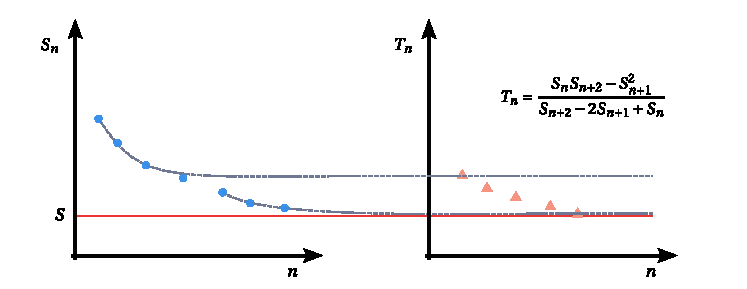
\includegraphics{figures/aitken}
  \caption{Geometrical interpretation of Aitken's \(\Delta^2\) method.}
  \label{fig:aitken}
\end{figure}

One can also show that if \((S_n)\) goes to its limit \(\S\) at a rate strictly greater than \(1\)\footnote{$(S_{n})$, ${n \in \mathbb{N}}$ converges linearly to $S$ if there exists a number $\mu \in(0,1)$ such that \(\lim_{n \rightarrow \infty} \frac{\left|S_{n+1}-S\right|}{\left|S_{n}-S\right|}=\mu\).}, \((T_n)\) does not have a better rate of convergence.

In practice, the sequence produced by Aitken's \(\Delta^2\) method tends to converge faster to the limit than \((S_n)\) does.
Very often, it is much cheaper to calculate \((T_n)\), which involves only the calculation of differences, one multiplication, and one division, than to calculate many more terms of the sequence \((S_n)\).
Care must be taken, however, to avoid introducing errors due to insufficient precision when calculating the differences in the numerator and denominator of the expression.

There is, however, no universal sequence accelerator capable of accelerating all sequences.
It is also the case that nonlinear transformations can even fail to converge or converge to a value other than the limit of the original sequence \citep{brezinski_extrapolation_2013}.

According to \cite{brezinski_extrapolation_2013}, there is a very strong connection between sequence transformations and fixed point methods for solving \(x= g( x)\), \(g\colon \mathbb R\to \mathbb R\).
The most well-known example of this connection is that between Aitken's \(\Delta^{2}\) process and Steffensen's method.
\begin{equation}
T_{n}=S_{n}-\frac{\left(S_{n+1}-S_{n}\right)^{2}}{S_{n+2}-2 S_{n+1}+S_{n}}, \quad n=0,1, \ldots \quad\text{for Aitken's process}
\end{equation}
and
\begin{equation}
x_{n+1}=x_{n}-\frac{\left(g\left(x_{n}\right)-x_{n}\right)^{2}}{g\left(g\left(x_{n}\right)\right)-2 g\left(x_{n}\right)+x_{n}},\quad n=0,1, \ldots \quad\text{for Steffensen's method.}
\end{equation}

Turning to vector sequences and systems of nonlinear equations, let \(F:(\mathbf w^{k}) \to(\mathbf y^{k})\) be a vector extrapolation method defined by
\begin{equation}
\mathbf y^k = F\left(\mathbf w^{k}, \ldots, \mathbf w^{k+m}\right), \quad n=0,1, \ldots
\end{equation}
For solving the fixed point problem \(\mathbf x=\pazocal S(\mathbf x)\) one can associate to it the iterative method
\begin{equation}
\mathbf x^{k+1}=F\left(\mathbf x^{k}, \pazocal S(\mathbf x^{k}), \ldots, \pazocal S^{m}(\mathbf x^{k})\right), \quad n=0,1, \ldots
\end{equation}
where \(\pazocal S^{m+1}(\mathbf x)=\pazocal S \circ \pazocal S^{m}(\mathbf x)\) and \(\pazocal S^{0}(\mathbf x)=\mathbf x\).
This approach is called full cycling or simply cycling.
Conversely to any fixed point iteration of this form, one can associate a sequence transformation of the previous form.
See Box~\ref{} for the general algorithm, excluding the extrapolation method.

There is a variety of vector extrapolation methods, where the major two categories are polynomial methods and methods based on the \(\epsilon\)-algorithm \citep{brezinski_extrapolation_2013, sidi_vector_2017}.
In this presentation, only the first category is considered since the second requires a relatively large number of function evaluations per iteration, making it unsuitable for the present use-case \citep{sidi_vector_2017}.

\cite{sidi_vector_2017} presents four different polynomial extrapolation methods.
They all attempt to exprress the limit of the vector sequence as a linear combination of the \(p\) previous iterates, as follows
\begin{equation}
\mathbf s \approx \mathbf{s}_{k, m}=\sum_{j=0}^{m} \gamma_{j} \mathbf w^{k+j},
\end{equation}
where \(\mathbf s\) is the limit of the vector sequence.
The methods to be presented next appear naturally when considering the vector sequence generated by
\begin{equation}
  \mathbf w^{k+1} = \mathbf{T}\mathbf w^k +\mathbf d,
\end{equation}
where \(\mathbf I - \mathbf T\) is non-singular.
It is tighly connected to the solution of linear systems of equations.
Considering the minimal polynomial of \(\mathbf T\) with respect to \(\Delta \mathbf w^{k} = \mathbf w^{k+1} -\mathbf w^k\) and \(\boldsymbol \epsilon^k = \mathbf w^k - \mathbf s\)\footnote{A polynomial \(P(\lambda)\) is said to be minimal with respect to a vector \(\mathbf a\), if \(P(\mathbf T) \mathbf a = 0\) and it of least degree.}, \(P(\lambda)\),
\begin{equation}
  P(\lambda ) = \sum_{j=0}^i c_j \lambda^j, \quad c_i=1,
\end{equation}
where \(i\) is the degree of the polynomial, the limit of the sequence can be found exactly as
\begin{equation}
  \mathbf s = \frac{ \sum_{j=0}^i c_j \mathbf w^{k+j}}{ \sum_{j=0}^i c_j}.
\end{equation}

This can be derived considering the definition of \(P(\lambda)\), \(P(\mathbf T) \boldsymbol \epsilon^k=0\).
Therefore,
\begin{equation}
\mathbf 0=P(\mathbf T) \boldsymbol \epsilon^{k}=\sum_{j=0}^{i} c_{j} \mathbf T^{j}  \boldsymbol\epsilon^{j}=\sum_{j=0}^{i} c_{j} \boldsymbol \epsilon^{k+j}.
\end{equation}
and so
\begin{equation}
0=\sum_{i=0}^{k} c_{i} \boldsymbol{\epsilon}_{n+i}=\sum_{i=0}^{k} c_{i} \boldsymbol{x}_{n+i}-\left(\sum_{i=0}^{k} c_{i}\right) \mathbf{s}.
\end{equation}
Solving this for \(\mathbf s\), one obtains the desired result, provided \(\sum_{j=0}^{i} c_{j} \neq 0\).

The coefficients of \(P(\lambda)\) can be computed considering
\begin{equation}
\mathscr W^{i-1} \mathbf c^{\prime}=-\Delta \mathbf w_{k+i}, \quad \mathbf c^{\prime}=\left[c_{0}, c_{1}, \ldots, c_{i-1}\right]^{T},
\end{equation}
where \(\mathscr W^i = [\Delta \mathbf w^k, \dots, \Delta \mathbf w^{k+i}]\), since from the defintion of \(P(\lambda)\), one has
\begin{equation}
  \mathbf 0 = P(\mathbf T) \Delta \mathbf w^k = \sum_{j=0}^i c_i \mathbf T^j \Delta \mathbf w^k = \sum_{j=0}^i c_i \Delta \mathbf w^{k+j}.
\end{equation}

The degree of \(P(\lambda)\) can be as large as the dimension of \(\mathbf w\).
Hence, to be practical, the minimal polynomial extrapolation (MPE), the reduced rank extrapolation (RRE), the modified minimal extrapolation (MMPE), and the single-value decomposition, minimal polynomial extrapolation (SVD-MPE) all choose a polynomial of a lesser degree.
The approximations are corresponding to each extrapolation method are presented in what follows.

\paragraph{MPE}

Solve the overdetermined linear system \(\mathscr W^{m-1} \mathbf c^{\prime}=-\Delta \mathbf w_{k+m}\) in the least-squares sense for \(\mathbf c^{\prime}=\left[c_{0}, c_{1}, \ldots, c_{m-1}\right]^{T}\).
This amounts to solving the optimization problem
\begin{equation}
\min _{c_{0}, c_{1}, \ldots, c_{p-1}}\left\|\sum_{j=0}^{m-1} c_{j} \Delta \mathbf w^ {k+j}+\Delta \mathbf w^{k+m}\right\|_2
\end{equation}
which can also be expressed as
\begin{equation}
  \min _{\mathbf c^{\prime}}\left\|\mathscr W^{m-1} \mathbf c^{\prime}+\mathbf w^{k+m}\right\|_2, \quad \mathbf c^{\prime}=\left[c_{0}, c_{1}, \ldots, c_{m-1}\right]^{T} .
\end{equation}
With \(c_{0}, c_{1}, \ldots, c_{k-1}\) available, set \(c_{m}=1\) and compute \(\gamma_{q}=c_{q} / \sum_{j=0}^{m} c_{j}, q=0,1, \ldots, m\), provided \(\sum_{j=0}^{m} c_{j} \neq 0\).

\paragraph{RRE}

Solve the overdetermined linear system \(\mathscr W^{m} \boldsymbol\gamma=0\) in the least-squares sense, subject to the constraint \(\sum_{j=0}^{m} \gamma_{j}=1\).
This amounts to solving the optimization problem
\begin{equation}
\min _{\gamma_{0}, \gamma_{1}, \ldots, \gamma_{m}}\left\|\sum_{j=0}^{m} \gamma_{j} \Delta\mathbf w^{k+j}\right\| \text { subject to } \sum_{j=0}^{m} \gamma_{j}=1
\end{equation}
which can also be expressed as
\begin{equation}
\min _{\boldsymbol\gamma}\left\|\mathscr W^{m} \boldsymbol\gamma\right\|_2 \quad \text { subject to } \sum_{j=0}^{m} \gamma_{j}=1 ; \quad \boldsymbol\gamma=\left[\gamma_{0}, \gamma_{1}, \ldots, \gamma_{m}\right]^{T} .
\end{equation}

\paragraph{MMPE}

Consider a set of \(m\) linearly independent vectors \(\mathbf q_j\), \(j=1, \dots, m\).
Solve the linear system
\begin{equation}
  \left(\mathbf q^{j}, \mathscr W^{m-1} \mathbf c^{\prime}\right)=-\left(\mathbf q^{j}, \Delta \mathbf w^{k+m}\right), \quad j=1, \ldots, m,
\end{equation}
which can also be expressed as
\begin{equation}
  \sum_{j=0}^{m-1}\left(\mathbf q_{j}, \Delta \mathbf w^{k+j}\right) \mathbf c_{j}=-\left(\mathbf q^{j}, \Delta \mathbf w^{k+p}\right), \quad j=1, \ldots, m.
\end{equation}
This is, in fact, a system of \(m\) linear equations for the \(m\) unknowns \(c_{0}, c_{1}, \ldots, c_{m-1}\).
With \(c_{0}, c_{1}, \ldots, c_{m-1}\) available, set \(c_{m}=1\) and compute \(\gamma_{q}=c_{q} / \sum_{j=0}^{m} c_{j}, i=0,1, \ldots, m\), provided \(\sum_{j=0}^{m} c_{j} \neq 0\).

\paragraph{SVD-MPE}

Solve the standard \(l_{2}\) constrained minimization problem
\begin{equation}
  \min_{\mathbf c}\left\|\mathscr W^{m} \mathbf c\right\|_{2} \quad \text { subject to }\|\mathbf c\|_{2}=1, \quad \mathbf c=\left[c_{0}, c_{1}, \ldots, c_{m}\right]^{T} .
\end{equation}
The solution \(\mathbf c\) is the right singular vector corresponding to the smallest singular value \(\sigma_{\min }\) of \(\mathscr W^{m}\), i.e., \({\mathscr W^{m}}^{*} \mathscr W^{m} \mathbf c=\sigma_{\min }^{2} \mathbf c\), \(\|\mathbf c\|_{2}=1\).
It is assumed that \(\sigma_{\min }\) is simple so that \(\mathbf c\) is unique up to a multiplicative constant \(\phi\), \(|\phi|=1\).

With \(c_{0}, c_{1}, \ldots, c_{m}\) available, compute \(\gamma_{q}=c_{q} / \sum_{j=0}^{m} c_{j}, q=0,1, \ldots, m\), provided \(\sum_{j=0}^{m} c_{j} \neq 0\).
The assumption that \(\sigma_{\min }\) is simple guarantees the uniqueness of the \(\gamma_{i}\).

\cite{sidi_vector_2017} also suggest cycling with frozen \(\gamma_i\), where after some iterations the \(\gamma_i\) are frozen and reused henceforth.
A parallel version of the full cycling procedure is also described.

\paragraph{Connection to Krylov subspace methods}

According to \cite{sidi_vector_2017}, the so-called Krylov subspace methods are closely related to the vector extrapolation methods presented above.
When the latter are applied to vector sequences obtained by applying fixed-point iterative methods to nonsingular linear systems of equations, they are mathematically equivalent.
More precisely, the MPE and the RRE methods are mathematically equivalent to the methods of Arnoldi and generalized minimal residual (GMR).

However, Krylov subspace methods and extrapolation methods differ in their algorithmic aspects entirely:
The only input of the former is a procedure that performs the matrix-vector multiplication without explicitly knowing the matrix coefficient matrix.
The latter take as their only input a vector sequence that results from a fixed-point iterative scheme without knowing the matrix coefficient matrix to know what the scheme is.

\cite{sidi_vector_2017} describes two different Newton-Krylov methods, the Newton-Arnoldi and the Newton-GMRES.
Nevertheless, these are not pursued here as they require a large amount of function evaluation per iteration of the Newton loop. They approximate the product of the Jacobian by a vector through a finite difference approach dependent on an arbitrarily small parameter \(\epsilon\).

In \cite{michler_interface_2005}, a Krylov-subspace method is proposed in the context of FSI.
However, as pointed out by \cite{kuttler_vector_2009}, the correct term for this approach should be instead a "Krylov-based vector extrapolation" method.
The method proposed can be obtained by applying the RRE to the sequence of residuals computed as
\(\Delta \mathbf r^*_i = \mathbf x^*_i - \mathbf x^k\), where the subscript \(i\) concerns the internal loop of the vector extrapolation method, and whose limit is \(\mathbf 0\).
\cite{kuttler_vector_2009} argues that these residual differences have unfavorable numerical properties and should be avoided.

% \begin{framedbox}[htbp]
%   \caption{Arnoldi process to orthonormalize temperature deltas}
%   \label{box:arnoldi_process}
%   \begin{center}
%     \begin{minipage}{0.9\textwidth}
%     \begin{enumerate}[(i)]
%       \item \(j=1\)
%       \item \(\Delta \bm\uptheta^*_m = \Delta \bm\uptheta^*_m - \Delta \bm\uptheta^*_j\frac{\Delta\bm\uptheta^*_m\cdot\Delta\bm\uptheta^*_j}{\Delta\bm \uptheta^*_j\cdot\Delta\bm\uptheta^*_j}\)
%       \item \(j=j+1\)
%       \item If \(j<m-1\) go to Step (ii)
%       \item \(\Delta\bm \uptheta^*_m = \Delta\bm\uptheta^*_m/\|\Delta \bm \uptheta^*_m\|\)
%     \end{enumerate}
%     \end{minipage}
%   \end{center}
% \end{framedbox}
%
% \begin{framedbox}[htbp]
%   \caption{Timestep \(n\) of the GMRES-inspired approach.}
%   \label{box:gmres_inspired}
%   \begin{center}
%     \begin{minipage}{0.9\textwidth}
%     \begin{enumerate}[(i)]
%     \item \(k=0\)
%     \item If no previous timesteps are to be reused or \(n=0\) then
%     \begin{itemize}
%       \item Clear all \(\Delta \bm \uptheta^*_i\), \(\Delta \mathbf r^*_i\)
%       \item \(m=0\)
%     \end{itemize}
%     \item \(\bm \uptheta^*_1 = \pazocal T\circ \pazocal U(\bm \uptheta^0)\)
%     \item \(\mathbf r^0 = \bm \uptheta^*_1 - \bm \uptheta^0\)
%     \item Enter the Newton loop
%     \begin{enumerate}[(1)]
%       \item If no previous iterations are to be reused
%       \begin{itemize}
%         \item Clear all \(\Delta \bm\uptheta^*_i\), \(\Delta \mathbf r^*_i\)
%         \item \(m=0\)
%         \item \(\xi = \|\mathbf r^*_k\|\)
%       \end{itemize}
%       else
%       \begin{itemize}
%         \item Compute \(\bar{\mathbf\alpha}\) (Equation~\eqref{eq:gmres_ls_condition}) and \(\xi\) (Equation~\eqref{eq:gmres_residual})
%         \item \(\bm \uptheta^*_{m+1} = \bm \uptheta^*_1\)
%       \end{itemize}
%       \item Enter the Krylov loop
%       \begin{enumerate}[(a)]
%         \item \(m=m+1\)
%         \item \(\Delta \bm\uptheta^*_m = \bm\uptheta^*_m - \bm\uptheta^k\)
%         \item Orthogonalize (Box~\ref{box:arnoldi_process}) and relax \(\Delta \bm\uptheta^*_m\) (Equation~\eqref{})
%         \item \(\bm\uptheta^*_m = \bm\uptheta^k + \Delta\bm\uptheta^*_m\)
%         \item \(\bm \uptheta^*_{m+1} = \pazocal T \circ \pazocal U(\bm \uptheta^*_m)\)
%         \item \(\Delta \mathbf r^*_m = (\bm\uptheta^*_{m+1} - \bm \uptheta^*_m) - \mathbf r^k\)
%         \item Compute \(\bar{\mathbf\alpha}\) (Equation~\eqref{eq:gmres_ls_condition}) and \(\xi\) (Equation~\eqref{eq:gmres_residual})
%         \item If convergence has not been reached, \(\xi>\epsilon_2\), go to Step (a)
%       \end{enumerate}
%     \item \(\bm\uptheta^{k+1} = \bm\uptheta^k + \sum_{i=1}^m \bar{\alpha}_i \Delta\bm\uptheta_i\)
%     \item \(k=k+1\)
%     \item \(\bm\uptheta^*_1 = \pazocal T\circ \pazocal U(\bm\uptheta^{k})\)
%     \item \(\mathbf r^k = \bm\uptheta^*_1 - \bm \uptheta^k\)
%     \item If convergence has not been reached, \(\|\mathbf r^k\| > \epsilon_1\), go to Step (1)
%     \end{enumerate}
%     \end{enumerate}
%     \end{minipage}
%   \end{center}
% \end{framedbox}

% \Floatbarrier

\section{Multipoint iteration functions with memory}

\begin{table}[htbp]
  \caption{Summary of the comparison between the FFT-Galerkin method.}
\label{tab:comparison_fft_galerkin_fem}
  % \setlength{\tabcolsep}{1pt}
  \centering
    \begin{tabular}{l cc p{3.5cm}}
    Method & \makecell[c]{Memory\\requirements} & \makecell[c]{Nr function\\evaluations\\per iteration} & Obs.\\
    \hline  \hline
    \multirow{3}{*}{\vphantom{\Big|}Fixed-point iteration} & \multirow{3}{*}{2 \((n\times 1)\) vectors} & \multirow{3}{*}{1} & \textbullet \textcolor{red!70!black}{Often diverges.}\\
    & & &\textbullet \textcolor{green!50!black}{Simplest method}.\\
    & & &\textbullet Memory efficient.\\
    \hline
    \multirow{3}{*}{Underrelaxation} & \multirow{3}{*}{2 \((n\times 1)\) vectors} & \multirow{3}{*}{1} & \textbullet Simple.\\
    & & &\textbullet Improved stability over fixed-point.\\
    & & &\textbullet Need to manually choose a relaxation parameter.\\
    \hline
    \multirow{3}{*}{Aitken relaxation} & \multirow{3}{*}{3 \((n\times 1)\) vectors} & \multirow{3}{*}{1} & \textbullet Very popular in FSI.\\
    & & & \textbullet Dynamic relaxation.\\
    & & & \textbullet Improved stability over fixed-point.\\
    \hline
    \multirow{3}{*}{Broyden's family} & \multirow{3}{*}{\makecell[c]{2 \((n\times 1)\) vectors\\2 \((n\times (m-1))\) matrices}} & \multirow{3}{*}{1} & \textbullet \\
    & & & \textbullet\\
    & & & \textbullet\\
    \hline
    \multirow{3}{*}{Anderson's family} & \multirow{3}{*}{\makecell[c]{2 \((n\times 1)\) vectors\\2 \((n\times (m-1))\) matrices}} & \multirow{3}{*}{1} & \textbullet \\
    & & & \textbullet\\
    & & & \textbullet\\
    \hline
    \multirow{3}{*}{\makecell[l]{Cycling with\\vector extrapolation}} & \multirow{3}{*}{\(m+2\) \((n\times 1)\) vectors} & \multirow{3}{*}{\(m+1\)} & \textbullet\\
    & & & \textbullet\\
    & & & \textbullet\\
  \hline\hline
  \multicolumn{4}{l}{\vphantom{\Huge |}\parbox{\textwidth}{\footnotesize{${}^*$ The inner loop of the strongly coupled scheme may converge very slowly or even diverge.}}}
  \end{tabular}
\end{table}

\begin{table}[htbp]
  \caption{Summary of the comparison between the FFT-Galerkin method.}
\label{tab:comparison_fft_galerkin_fem}
  % \setlength{\tabcolsep}{1pt}
  \centering
    \begin{tabular}{l c}
    Method & Update formula\\
    \hline\hline
    \vphantom{\Huge |}Fixed-point &  \makecell[l]{\(\mathbf x^{k+1} = \mathbf x^k -  \pazocal R^k\)}\\
    \hline
    Underrelaxation & \makecell[l]{\vphantom{\Huge |}\(\mathbf x^{k+1} = \mathbf x^k - \omega\pazocal R^k\),\\\(0<\omega<1\).}\\
    \hline
    Aitken relaxation & \makecell[l]{\vphantom{\Huge |}\(\mathbf x^{k+1} = \mathbf x^k - \omega^{(k)}\pazocal R^k\),\\    \(\omega^{(k)}=-\omega^{(k-1)} \displaystyle\frac{\left(\mathbf{r}^{(k)}-\mathbf{r}^{(k-1)}\right)^{\mathrm{T}} \mathbf{r}^{(k-1)}}{\left(\mathbf{r}^{(k)}-\mathbf{r}^{(k-1)}\right)^{2}}.\)
    }\\
    \hline
    Broyden's family & \makecell[l]{\vphantom{\Huge |} \(\mathbf x^{k+1} = \mathbf x^{k}- \left(G_\pazocal R^{k-m} +\left(\mathscr{X}^{k}-G_\pazocal R^{k-m} \mathscr{R}^{k}\right){\mathbf V^k}^T\right) \pazocal R^k,\)\\
    \({\mathbf V^k}^T = {\mathbf M^k}^{-1}{\mathbf N^k}^T\),\\
    Type I:  \({M^k} = {\mathscr X^k}^T G_\pazocal R^k \mathscr R^k,\quad {N^k}^T = {\mathscr X^k}^T G_\pazocal R^k,\)\\
    Type II: \({M^k} = {\mathscr R^k}^T \mathscr R^k,\quad {N^k}^T = {\mathscr R^k}^T\)\\
    {\small \(\mathbf V^k\) is usually computed using \(QR\)-decomposition.}
    }\\
    \hline
    Anderson's family & \makecell[l]{\vphantom{\Huge |} \(\mathbf x^{k+1} = \mathbf x^{k} -\left(-\beta \mathbf I+\left(\mathscr{X}^{k}+\beta \mathscr{R}^{k}\right){\mathbf V^k}^T\right) \pazocal R^k,\)\\
    \({\mathbf V^k}^T = {\mathbf M^k}^{-1}{\mathbf N^k}^T\),\\
    Type I:  \({M^k} = {\mathscr X^k}^T \mathscr R^k,\quad {N^k}^T = {\mathscr X^k}^T ,\)\\
    Type II: \({M^k} = {\mathscr R^k}^T \mathscr R^k,\quad {N^k}^T = {\mathscr R^k}^T\)\\
    {\small \(\mathbf V^k\) is usually computed using \(QR\)-decomposition.}
    }\\
    \hline
    \makecell[l]{Cycling with\\ vector extrapolation} & \makecell[l]{\vphantom{\Huge |}
    \(\mathbf x^{k+1} = \sum_{j=0}^m \gamma_j \pazocal S^{i+j}(\mathbf x^k)\),\\
    \(\gamma_q = c_q/\sum_j c_j,\quad q=0,1,\dots,m,\)\\
    \textbf{MPE}: \(\mathbf c ' = [c_0,c_1,\dots,c_{m-1}]^T = \arg \min_{\bar{\mathbf c}} \left\|\mathscr S^{m-1} \bar{\mathbf c}^\prime + \pazocal S^{i+m}(\mathbf x^k)\right\|_2\),\\
    \(c_m=1\),\\
    \textbf{RRE}: \(\boldsymbol{\gamma} = [\gamma_0,\gamma_1,\dots,\gamma_{m}]^T = \arg \min_{\bar{\boldsymbol{ \gamma}}} \left\|\mathscr S^{m} \hat{\boldsymbol{\gamma}}\right\|_2\),\\
    Subject to \(\sum_{j=0}^m \gamma_j =1\).\\
    \textbf{MMPE}: \(\left(\mathbf q^{j}, \mathscr S^{m-1} \mathbf c^{\prime}\right)=-\left(\mathbf q^{j}, \Delta \mathbf S^{i+m}(\mathbf x^k)\right), \quad j=1, \ldots, m,\)\\
    for a set of \(m\) linearly independent vectors \(\mathbf q_j\), \(j=1, \dots, m\).\\
    \(\mathbf c ' = [c_0,c_1,\dots,c_{m-1}]^T.\)\\
    \textbf{SVD-MPE}: \(\mathbf c = \arg\min_{\bar{\mathbf c}}\left\|\mathscr S^{m} \bar{\mathbf c}\right\|_{2} \quad \text { subject to }\|\bar{\mathbf c}\|_{2}=1,\)\\
    \(\mathbf c=\left[c_{0}, c_{1}, \ldots, c_{m}\right]^{T}\).
    }\\
  \hline\hline
  \end{tabular}
\end{table}
